\documentclass[a4paper,12pt]{article}
\usepackage[ngerman]{babel}
\usepackage{ucs}
\usepackage{multirow}
\usepackage{xltxtra}
\usepackage[utf8x]{inputenc}
\usepackage{fontspec}
\usepackage[automark]{scrpage2}
\usepackage{eurosym}
\usepackage{graphicx}
\usepackage[paper=a4paper,left=25mm,right=25mm,top=25mm,bottom=25mm]{geometry}
\usepackage[normalem]{ulem}
\pagestyle{scrheadings}
\setmainfont[Mapping=tex-text]{Liberation Serif}
\clearscrheadfoot
\providecommand\roboravelanguage{en}
\begin{document}
\ohead{Last edit: \today}
\title{Rules a-MAZE-ing Challenge 2020}
\makeatletter
\let\inserttitle\@title
\makeatother
 \begin{center}

\includegraphics[width=0.5\textwidth]{logo.png}

\huge                      % Schriftgröße einstellen
\bfseries                   % Fettdruck einschalten
\inserttitle
  \end{center}
This is only an unofficial translation. In case of doubt, only the refeere's interpretation of the newest
official german rules will count. Differences to the 2018 rules are marked in \textbf{bold}.

\section{Goal}
Design, build and program a robot that can follow a raised wooden maze withoutfalling
off. Completing the maze before the time limit adds Bonus Points to your score.

\section{Who Can Play}
Teams of 2 to 4 players in separate divisions for:
\begin{itemize}
	\item Middle School (Age 10-13)
	\item High School (Age 14-17)
\end{itemize}

\section{Required Materials}
Autonomous robot, any platform, costing \euro{ 1500} or less, and meets the following design cons-
traints, which will be verified during Check-In:
\begin{itemize}
\item Robot is not allowed to use any sensors to assist it in following the maze, wheel encoders
are allowed. Gyroscopes or similar sensors also count as sensors.
\textbf{If sensors are present on the robot, they must be deactivated by totally unplugging all
cables for power or data transfer to the sensor.}
\item Volume of the robot must not exceed 65030 cubic cm.
\end{itemize}

\section{General Rules of Play}
\begin{itemize}
\item The robot has 2 minutes to complete the maze.
\item Within these 2 minutes you can do as many trials as you want. 
\textbf{A new trial can only be started if the robot has fallen off the maze.}
\item \textbf{A robot is considered to have fallen-off the maze when any of its wheels are
\emph{completely} off the surface of the maze.}
\item Only the trial with the
highest number of points will be counted.
\end{itemize}

\section{Challenge Specifications}
\begin{itemize}
\item The a-MAZE-ing tracks will all be identical and are constructed of wood that is approximately
24 cm wide and 2 cm tall.
\item There are various lengths, as determined by the division, with angles
of any combination of 45, 90, and 135 degrees that can turn in either direction.
\item \textbf{The allowed alignments are shown in the picture. \\}
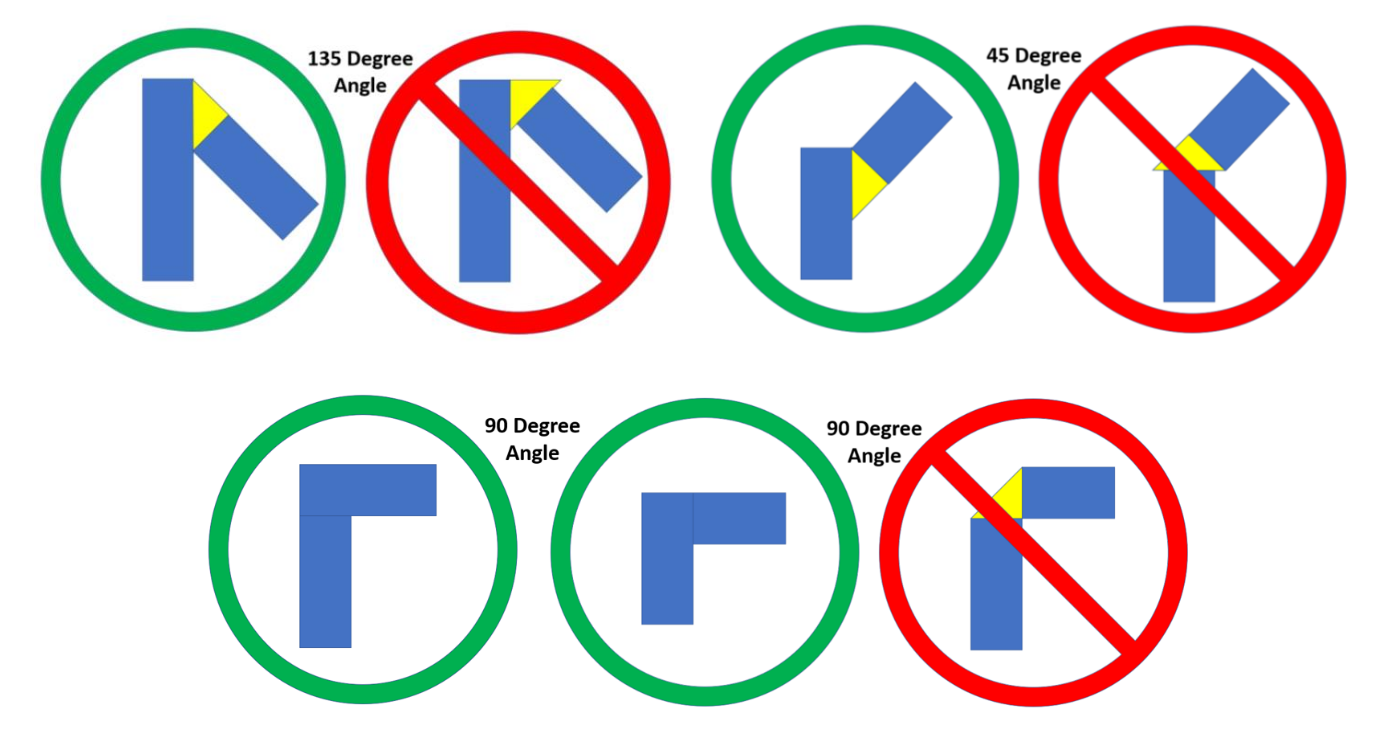
\includegraphics[width=1.0\textwidth]{amazeing_allowed.png}
\item \textbf{The pieces are typically taped together with heavy duct tape. However, they could be
joined with screws or glued splines. Regardless of the method used, every effort will be
made to ensure tracks are as smooth and free of irregularities as possible.}
\item \textbf{The referees will determine if there will be separate tracks for all divisions or if all
divisions will use the same track with marks for the different finishing lines.}
\item Tracks for the different divisions:
\begin{itemize}
\item Middle School Division – Finish line will be halfway between the 5th and 6th angled turn
\item High School Division – Finish line is at the end of the track
\end{itemize}
\item \textbf{The lines marking the end of a straight or turn can be seen in the following picture.\\}
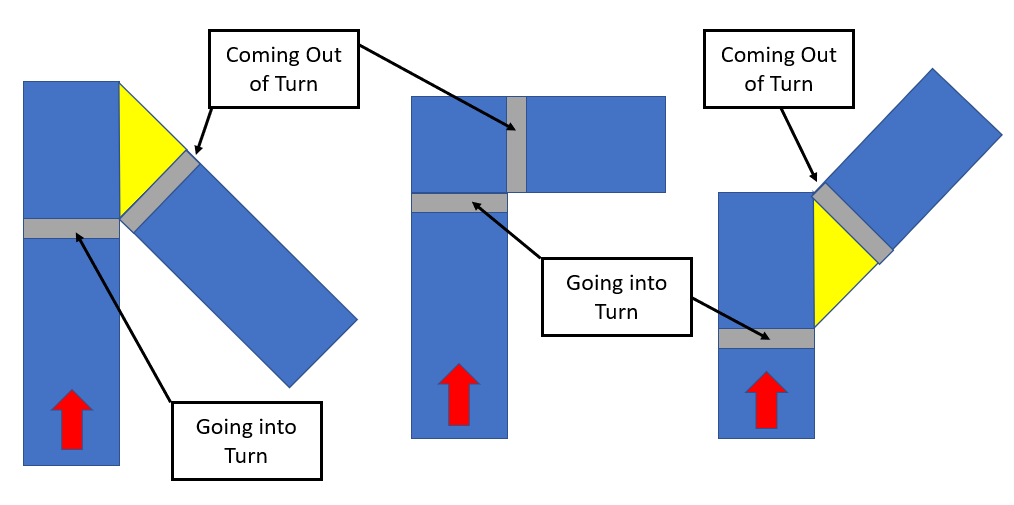
\includegraphics[width=1.0\textwidth]{amazeing_angle.png}
\end{itemize}

\section{Scoring period}
\par The way the earned points are counted for the challenge will be announced on the first day of the event.

\section{Scoring}
\begin{itemize}
\item Each completed straight-away is worth 50 points and each completed angle is worth 100 points.
\item \textbf{A straight-away or angle counts as finished when any part of the robot has crossed th finishing line.}
\item If the robot falls off the maze before reaching the finish line, then the run is concluded, and the score received
includes any portion of the maze that is completed in it’s entirety, but no time bonus points are awarded.
\item \emph{Time bonus} points are only awarded if the robot reaches the finish line before the 120 seconds ends. Any
remaining time is then added to the maze score as a time bonus point value (the whole number part of the
time).
\end{itemize}
\section{Scoring Matrix}
\begin{center}
\begin{tabular}{|c|c|c|c|c|c|c|c|c|} \hline
	\multirow{2}*{Division} & 1. & 1. & 2. & 2. & 3. & 3. & 4. \\
	& Straight & Turn & Straight &Turn & Straight &Turn & Straight   \\ \hline
	MS (10-13) & 50 & 100 & 50 & 100 & 50 & 100 & 50   \\ \hline
	Sum MS & 50 & 150 & 200 & 300 & 350 & 450 & 500   \\ \hline
	HS (14-17) & 50 & 100 & 50 & 100 & 50 & 100 & 50  \\ \hline
	Sum HS & 50 & 150 & 200 & 300 & 350 & 450 & 500   \\ \hline
\end{tabular} \\ \vspace{\baselineskip}
\begin{tabular}{|c|c|c|c|c|c|c|c|c|} \hline
	\multirow{2}*{Division} & 4. & 5. & 5. & 6. & 6. & 7. \\
	& Turn & Straight & Turn & Straight & Turn & Straight     \\ \hline
	MS (10-13) & 100 & 50 & 100 & 50 & &  \\ \hline
	Sum MS & 600 & 650 & 750 & 800 &  &     \\ \hline
	HS (14-17) & 100 & 50 & 100 & 50 & 100 & 50   \\ \hline
	Sum MS & 600 & 650 & 750 & 800 & 900  & 950    \\ \hline
\end{tabular}
\end{center}
\end{document}
